\documentclass[../../main]{subfiles}

\begin{document}

\newcommand\centerImage[1]{
\begin{tabular}{@{}c@{}}
#1
\end{tabular}
}
\newcommand\addCharts[4][0]{
    \draw[dotted, black!50!white] (0,0) circle[radius=1];
    \pgfmathsetmacro{\startAngle}{#1};
    \pgfmathsetmacro{\n}{#2};
    \pgfmathsetmacro{\d}{#3};
    \pgfmathsetmacro{\singleAngle}{360 / \d};
    \foreach \i in {1,...,\n}{
        \pgfmathsetmacro{\angle}{\startAngle+\i * \singleAngle};
        \pgfmathsetmacro{\prevAngle}{\startAngle+(\i - 1) * \singleAngle};
        \fill[#4] (0,0) -- (\angle:1) arc (\angle:\prevAngle:1) -- cycle;
        \draw[black] (0,0) -- (\angle:1) arc (\angle:\prevAngle:1) -- cycle;
        
    }
    \foreach \i in {0,...,\n}{
        \pgfmathsetmacro{\angle}{\startAngle+\i * \singleAngle};
        \draw[-] (0,0) -- (\angle:1);
    }
    \foreach \i in {1,...,\n}{
        \pgfmathsetmacro{\angle}{\startAngle+(\i - 1) * \singleAngle};
        \node[] at (\angle + .5 * \singleAngle:.5) {$\frac{1}{\d}$};
    }
}
\newcommand\addDottedCharts[4][0]{
    \draw[dotted, black!50!white] (0,0) circle[radius=1];
    \pgfmathsetmacro{\startAngle}{#1};
    \pgfmathsetmacro{\n}{#2};
    \pgfmathsetmacro{\d}{#3};
    \pgfmathsetmacro{\singleAngle}{360 / \d};
    \foreach \i in {1,...,\n}{
        \pgfmathsetmacro{\angle}{\startAngle+\i * \singleAngle};
        \pgfmathsetmacro{\prevAngle}{\startAngle+(\i - 1) * \singleAngle};
        \fill[#4] (0,0) -- (\angle:1) arc (\angle:\prevAngle:1) -- cycle;
        \draw[dotted, black] (0,0) -- (\angle:1) arc (\angle:\prevAngle:1) -- cycle;
        
    }
    \foreach \i in {0,...,\n}{
        \pgfmathsetmacro{\angle}{\startAngle+\i * \singleAngle};
        \draw[dotted] (0,0) -- (\angle:1);
    }
    \foreach \i in {1,...,\n}{
        \pgfmathsetmacro{\angle}{\startAngle+(\i - 1) * \singleAngle};
        \node[] at (\angle + .5 * \singleAngle:.5) {$\frac{1}{\d}$};
    }
}
\newcommand\drawChartDiagram[4][0]{
\begin{tikzpicture}[scale=1.75]
    \draw[dotted, black!50!white] (0,0) circle[radius=1];
    \pgfmathsetmacro{\startAngle}{#1};
    \pgfmathsetmacro{\n}{#2};
    \pgfmathsetmacro{\d}{#3};
    \pgfmathsetmacro{\singleAngle}{360 / \d};
    \foreach \i in {1,...,\n}{
        \pgfmathsetmacro{\angle}{\startAngle+\i * \singleAngle};
        \pgfmathsetmacro{\prevAngle}{\startAngle+(\i - 1) * \singleAngle};
        \fill[#4] (0,0) -- (\angle:1) arc (\angle:\prevAngle:1) -- cycle;
        \draw[black] (0,0) -- (\angle:1) arc (\angle:\prevAngle:1) -- cycle;
        
    }
    \foreach \i in {0,...,\n}{
        \pgfmathsetmacro{\angle}{\startAngle+\i * \singleAngle};
        \draw[-] (0,0) -- (\angle:1);
    }
    \foreach \i in {1,...,\n}{
        \pgfmathsetmacro{\angle}{\startAngle+(\i - 1) * \singleAngle};
        \node[] at (\angle + .5 * \singleAngle:.5) {$\frac{1}{\d}$};
    }
    \end{tikzpicture}
}

In den bisherigen Kapiteln haben wir es fast ausschließlich mit ganzen Zahlen, also $1,2,3,\dots$, zu tun gehabt. Wir können solche Zahlen addieren, subtrahieren, dividieren und multiplizieren. Außerdem kennen wir bereits einige Rechengesetze wie das Kommutativgesetz.

Das Problem bei den ganzen Zahlen besteht darin, dass wir, wenn wir sie durcheinander teilen, sogenannte Dezimalbrüche erhalten, also Zahlen mit Nachkommastellen.
\begin{example}{}
\[3:5=0.6\]
\end{example}
Das Rechnen mit diesen ist nicht besonders angenehm. Wir führen deswegen eine neue Schreibweise für Divisionen ein:
\begin{definition}{Bruch}
Wir schreiben die Division zweier Zahlen $a$ und $b$ als Bruch \[a:b=:\frac{a}{b}\]
Dabei wird der Dividend über den Bruchstrich geschrieben und heißt \textbf{Zähler}. Der Divisor wird unter den Bruchstrich geschrieben und heißt \textbf{Nenner}.
\end{definition}
\noindent Brüche werden oft im richtigen Leben angewandt, z.B. wenn zwei Freunde sich eine Pizza teilen. Dann erhält jeder \emph{eine halbe} Pizza, als Bruch $\frac{1}{2}$. Gängig sind Brüche auch bei Zeit. Eine volle Stunde hat 60 Minuten. Oft nutzt man für 30 bzw. 15 Minuten die Ausdrücke eine \textbf{halbe} bzw. eine \textbf{Viertel}stunde.
\begin{example}{}
Wir wollen ausrechnen, wie viele Minuten eine Drittelstunde hat. Wir wissen, dass eine Stunde 60 Minuten hat. Wir rechnen also $60:3=20$ und haben das Ergebnis, dass eine Drittelstunde 20 Minuten dauert. Das Ergebnis können wir auch als Bruch aufschreiben: $20=\frac{60}{3}$ (da der Bruchstrich für ein Divisionszeichen steht).
\end{example}
\noindent Hinter einem Bruch verbirgt sich also immer einfach eine Zahl. Aus diesem Grund kann man mit Brüchen auch genauso rechnen wie mit Zahlen. Wir werden uns in diesem Kapitel anschauen, wie man sie addiert, subtrahiert, dividiert und multipliziert. Außerdem gibt es mit dem \textbf{Erweitern und Kürzen} zwei sehr praktische Hilfsmittel, die wir oft verwenden werden.

\subsection*{Übungsaufgaben}
Stelle die folgenden Zusammenhänge als Brüche dar und berechne jeweils ihren Wert.
\begin{enumerate}
    \item Jan ist heute morgen einen halben Kilometer zur Schule gelaufen.
    \item Ich bin gestern 9 Bahnen geschwommen, mein kleiner Bruder nur halb so weit.
    \item Meine Schwester hat sich mit fünf Freundinnen drei Pizzen geteilt.
\end{enumerate}

\section{Begriffe}
Zunächst wollen wir uns ein paar wichtige Begrifflichkeiten in Zusammenhang mit Brüchen anschauen und veranschaulichen, was Zähler und Nenner eines Bruches über ihn aussagen.
\begin{figure}[hbt]
    \centering
    \drawChartDiagram{4}{4}{blue!20!white}
    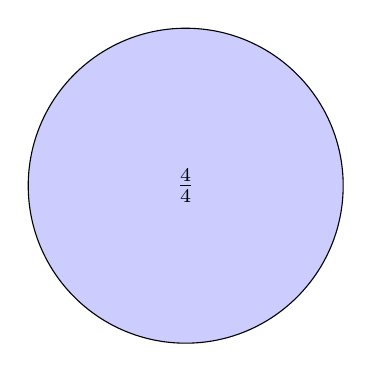
\begin{tikzpicture}[scale=2]
    \filldraw[fill=blue!20!white, draw=black] (0,0) circle[radius=1];

    \node[] at (0:0) {$\frac{4}{4}$};
    \end{tikzpicture}
    
    \[\frac{1}{4}+\frac{1}{4}+\frac{1}{4}+\frac{1}{4}=\frac{4}{4}\]
    
    \caption{Brüche stellen gleichgroße Anteile des Ganzen dar}
    \label{fig:fractions}
\end{figure}
Wir haben in der Einführung bereits zerteilbare \glqq Ganze\grqq~gesehen, zum Beispiel einen Kilometer, eine Stunde, einen Liter Milch oder Pizzen. Mithilfe von Brüchen zerteilen wir dieses \textbf{Ganze} in gleichgroße Teile. In wie viele, gibt der \textbf{Nenner} des Bruches (unter dem Bruchstrich) an. Im Bild haben wir den Kreis in 4 gleichgroße Teiler zerlegt, also ist der Nenner 4, während das Ganze der gesamte Kreis ist.
\[\frac{\colorobrace{5}{\text{Zähler}}}{\colorbrace{7}{\text{Nenner}}}\]
Allein dadurch, dass wir wissen, in wie viele Teile wir das Ganze zerlegt haben, können wir aber noch nicht sagen, welchen Teil des Ganzen wir nun tatsächlich haben: Die Information, wie viele dieser Teile wir nun wirklich haben, gibt uns der \textbf{Zähler} (über dem Bruchstrich). Weil wir vier Teile haben, ist auch der Zähler im Bild 4.

Jeder Bruch bezieht sich auf ein Ganzes. Wenn man mit Brüchen rechnet, sollte man sich also immer darüber im klaren sein, was das Ganze ist. Das ergibt sich entweder aus dem Sachzusammenhang oder, falls es keinen direkten Sachzusammenhang gibt, ist das Ganze einfach die Zahl $1$.

Ebenfalls sollte man beim Rechnen mit Brüchen immer im Hinterkopf behalten, dass der Bruchstrich für eine Division steht, man könnte also jederzeit den Zähler durch den Nenner teilen und dadurch eine Dezimalzahl (also mit Komma) erhalten.

\subsection*{Übungsaufgaben}
\begin{enumerate}
    \item Arne, Fabian und Timon machen ein Wettrennen über eine Strecke von 24 Kilometern. Nach einer Stunde hat Arne die Hälfte zurückgelegt, Timon hat $\frac{3}{8}$ der Strecke zurückgelegt und Fabian ist 
    \begin{enumerate}
        \item 1
        \item 2
        \item 3
        \item 4
    \end{enumerate}
    \item Auf einem Schreibtisch steht eine Blumenvase aus Ton. Versehentlich wird sie eines Tages vom Tisch gestoßen und zerspringt am Boden in neun gleichmäßige Scherben. Leider sind einige Stücke nicht mehr zu finden, sodass nur fünf Stücke wiedergefunden werden.
    \begin{enumerate}
        \item Gib den Anteil der wiedergefundenen Scherben als Bruch an.
        \item Was ist bei diesem Bruch das Ganze?
    \end{enumerate}
\end{enumerate}

\section{Unechte Brüche und Gemischte Zahlen}

Nachdem wir ein Grundverständnis für die Funktion von Brüchen bekommen haben, wollen wir uns als nächstes ein wenig genauer ansehen, welche Werte ein Bruch annehmen kann. Wenn man darüber redet, etwas sei ein Bruchteil von etwas anderem, dann reden wir normalerweise über einen wirklich kleineren Teil. Ein Bruchstück von einer Blumenvase, die zu Boden gefallen ist, ist zum Beispiel ein kleiner Teil der gesamten Vase. Letztlich kommt das Wort \glqq Bruch\grqq{} von der Vorstellung, ein großes Ganzes in gleich große Stücke zu zerbrechen.

Mathematische Brüche hingegen müssen nicht immer weniger als ein Ganzes sein. Bleiben wir bei der zerbrochenen Vase. Wenn wir davon ausgehen, dass die Vase in sieben gleich große Stücke zerbrochen ist und wir es schaffen, sechs Stücke wiederzufinden, haben wir insgesamt $\frac{6}{7}$ der Vase wiedergefunden: Von den sieben Stücken, die es insgesamt gab (Nenner, untere Zahl) sind sechs tatsächlich noch vorhanden (Zähler, obere Zahl). Wir haben also nur einen Bruchteil der Vase wiedergefunden.

Stellen wir uns nun aber vor, wir hätten neun Stücke gefunden. Da schon sieben Stücke eine ganze Vase ergeben, hätten wir mehr als nur eine Vase gefunden. Das entspricht nicht unserer Vorstellung, die wir bisher hatten, entspricht aber dem Bruch $\frac{9}{7}$.

Aus mathematischer Sicht gibt es kein Problem damit, auch solche Brüche zu verwenden, allerdings sind sie dann nicht mehr Teil eines einzigen Ganzen. Wenn es mehr Teile gibt als ein Ganzes, haben wir es nicht mit Bruchstücken \textit{eines} Ganzen zu tun. Brüche, in denen es mehr Bruchstücke gibt als nötig sind, um ein Ganzes zu erhalten, sind daher keine echten Brüche. Wir nennen sie \textbf{unechte Brüche}. Im Kontrast dazu nennen wir Brüche, die tatsächlich nur Teil \textit{eines} Ganzen sind, \textbf{echte Brüche}.

\begin{definition}{}
Ein Bruch $\frac{a}{b}$ heißt \textbf{echter Bruch}, wenn $a\leq b$, sonst heißt er \textbf{unechter Bruch}.
\end{definition}



\section{Erweitern und Kürzen}
\begin{figure}[htb]
    \centering
    \drawChartDiagram{3}{4}{red!20!white}
    \drawChartDiagram{6}{8}{yellow!20!white}
    \drawChartDiagram{9}{12}{blue!20!white}
    
    \[\frac{3}{4}=\frac{6}{8}=\frac{9}{12}\]
    \caption{Die Größe der Stücke verändert den Gesamtwert nicht}
    \label{fig:piece_size}
\end{figure}
\begin{theorem}{}
Ein Bruch kann erweitert bzw. gekürzt werden, indem man Zähler und Nenner mit der gleichen Zahl multipliziert bzw. durch die gleiche Zahl teilt. Dabei bleibt sein Wert unverändert.
\end{theorem}
Erweitern und Kürzen ändert den Wert des Bruches nicht. An der Abbildung sieht man, dass man keine neuen \glqq Stücke\grqq~hinzufügt, sondern (beim Erweitern) lediglich die vorhandenen Stücke in mehrere Stücke aufteilt oder (beim Kürzen) mehrere Stücke zu einem Stück zusammenfügt.

\begin{example}{}
Wenn wir den Bruch $\frac{4}{6}$ mit der Zahl 3 erweitern, erhalten wir $\frac{4\cdot 3}{6\cdot 3}=\frac{12}{18}$. Wir können Zähler und Nenner jederzeit separat umformen, also zu einem Produkt auseinanderziehen: $\frac{12}{18}=\frac{2\cdot 6}{3\cdot 6}$ (da Zähler und Nenner jeweils Zahlen, wie wir sie schon kennen, sind und wir deshalb mit ihnen genauso wie mit normalen Zahlen umgehen können). Nun sehen wir aber, dass sowohl in Zähler und Nenner eine 6 vorkommt, also können wir den Bruch gut durch 6 kürzen: $\frac{2\cdot 6}{3\cdot 6}=\frac{2}{3}$.
\end{example}

\section{Addition und Subtraktion von Brüchen}
In diesem Abschnitt wollen wir Brüche addieren und subtrahieren. Die Hauptschwierigkeit liegt hier darin, dass wir Brüche mit unterschiedlichem Nenner addieren können müssen, wir uns aber immer für einen Nenner entscheiden müssen.

Wir fangen mit dem einfachen Fall an: Wenn wir zwei Brüche mit \textbf{gleichem Nenner} addieren, dann haben wir bei beiden Brüchen dieselbe \glqq Stückgröße\grqq~, d.h. wir können die Zähler einfach addieren.
\begin{example}{}
\centerImage{\drawChartDiagram{2}{7}{red!20!white}}
$+$
\centerImage{\drawChartDiagram{4}{7}{red!20!white}}
$=$
\centerImage{\drawChartDiagram{6}{7}{red!20!white}}

\[\frac{2}{7}+\frac{4}{7} = \frac{2+4}{7}=\frac{6}{7}\]
\end{example}

Schwieriger wird es, wenn wir verschieden große Stücke addieren müssen. In diesem Fall bekommen wir nämlich ein neues Stück, das sich aus verschieden großen Stücken zusammensetzt, und können es nicht durch einen einzigen Bruch darstellen. Aus diesem Grund verkleinern wir alle Stücke so, dass wir wieder nur gleichgroße Stücke haben.\\
Mathematisch heißt das, dass wir einen \textbf{Hauptnenner} suchen, also einen Nenner, den wir bei beiden Brüchen erreichen, wenn wir sie mit entsprechenden Zahlen erweitern.
\begin{example}{}
\centerImage{\drawChartDiagram{1}{3}{orange!20!white}}
$+$
\centerImage{\drawChartDiagram{1}{4}{blue!20!white}}
$=$
\centerImage{
\begin{tikzpicture}[scale=2]
    \addCharts{1}{3}{orange!20!white};
    \addCharts[120]{1}{4}{blue!20!white};
\end{tikzpicture}
}

\[\frac{1}{3}+\frac{1}{4}=~?\]

Nun suchen wir einen Hauptnenner, in diesem Fall $4\cdot 3=12$, und erweitern beide Brüche:\\

\centerImage{\drawChartDiagram{4}{12}{orange!20!white}}
$+$
\centerImage{\drawChartDiagram{3}{12}{blue!20!white}}
$=$
\centerImage{
\begin{tikzpicture}[scale=2]
    \addCharts{4}{12}{orange!20!white};
    \addCharts[120]{3}{12}{blue!20!white};
\end{tikzpicture}
}

\[\frac{1}{3}+\frac{1}{4}\ensuremath{\stackrel{\text{(Erweitern)}}{=}}\frac{4}{12}+\frac{3}{12}=\frac{4+3}{12}=\frac{7}{12}\]
\end{example}

Wenn wir Brüche subtrahieren wollen, verfahren wir genauso. Der einzige Unterschied ist, dass wir aus dem $+$ ein $-$ machen, die Stücke also nicht zu den anderen dazulegen, sondern entsprechend viele Stücke entfernen.
\begin{example}{}
\centerImage{\drawChartDiagram{4}{12}{orange!20!white}}
$-$
\centerImage{\drawChartDiagram{3}{12}{blue!20!white}}
$=$
\centerImage{
\begin{tikzpicture}[scale=2]
    \addCharts{1}{12}{orange!20!white};
    \addDottedCharts[30]{3}{12}{black!10!white};
\end{tikzpicture}
}

\[\frac{1}{3}-\frac{1}{4}\ensuremath{\stackrel{\text{(Erweitern)}}{=}}\frac{4}{12}-\frac{3}{12}=\frac{4-3}{12}=\frac{1}{12}\]
\end{example}

\begin{theorem}{Addition und Subtraktion von Brüchen}
Für zwei Brüche, $\frac{a}{b}$ und $\frac{c}{d}$, berechnet man die Summe/Differenz $\frac{a}{b}\pm\frac{c}{d}$ mit den folgenden Schritten:
\begin{enumerate}
    \item Beide Brüche auf einen Hauptnenner bringen, also den linken Bruch mit $d$ und den rechten mit $b$ erweitern:\[\frac{ad}{bd}\pm\frac{bc}{bd}\]
    \item Die Brüche auf einen Bruchstrich zusammenführen:\[\frac{ad\pm bc}{bd}\]
    \item Die Summe/Differenz im Zähler ausrechnen.
\end{enumerate}
\end{theorem}

\section{Multiplikation von Brüchen}
\begin{theorem}{Multiplikation von Brüchen}
Für zwei Brüche, $\frac{a}{b}$ und $\frac{c}{d}$, berechnet man das Produkt $\frac{a}{b}\cdot\frac{c}{d}$, indem man die Zähler und Nenner separat miteinander multipliziert:
\[\frac{a}{b}\cdot\frac{c}{d}=\frac{a\cdot c}{b\cdot d}\]
\end{theorem}
\section{Division von Brüchen}

\end{document}